\section{Overview}

As previously stated, the first two main goals of this thesis are to implement and deploy tools for deep clustering of motion tracking time series. In this context, DeepOF (deep Open Field) is a Python package that implements tools for loading, processing, and analyzing motion-tracking data. In particular, it provides two analysis pipelines for users to explore: a supervised pipeline, which aims to extract a set of pre-defined patterns from tracked animal trajectories, and an unsupervised pipeline, which applies state-of-the-art deep clustering to segment behavior over time. Moreover, the tool also includes a set of functions to explore the output of these analyses, including pattern expression enrichment and dynamics across experimental conditions, fitting normative models, exploring global shifts in behavior across time, and more. The current chapter includes a paper published in the \emph{Journal of Open Source Software} (JOSS), accepted for publication after a peer-review process that tested both the content of the paper and the proper functioning and writing of the deployed code \cite{Miranda2023DeepOF:Data}. At the moment of submitting this thesis, the latest stable version of the package is 0.4.6.

\section{Package design}

DeepOF was implemented following a modular design, with three modules intended for user interaction, called \python{deepof.data}, \python{deepof.post\_hoc}, and \python{deepof.visuals}. The first one deals with data loading, preprocessing, and pattern extraction. The second one provides a set of tools for post-hoc analysis of results obtained with the provided annotation pipelines, and the third one includes a plethora of visualization functions. A set of five extra modules contain models and utilities that are not intended for the user to access directly, but are consistently loaded by classes and functions in the public API.

Moreover, DeepOF includes a set of automatic tests deployed with continuous integration (CI), which makes it easier to make sure that all deployed code works as intended. Test coverage is reported automatically as well, to make it easier for maintainers to keep track of what is being tested if the codebase is extended. Extensive documentation is included too (both automatic for the API and manually generated for installation, examples, and tutorials), as well as contributing guidelines and a code of conduct. The language of choice (Python) was selected as the gold standard and most familiar tool for both data science libraries used to implement our models, and the behavioral analysis community as a whole.

All in all, DeepOF was implemented following best practices to make it maintainable and extensible in the future, and we believe it has the potential required to last in the field as a useful and easily accessible tool.

\section{Contribution to the work}

I am to date the sole contributor to the API design and code implementation of the DeepOF package. I also wrote the entirety of the included paper.

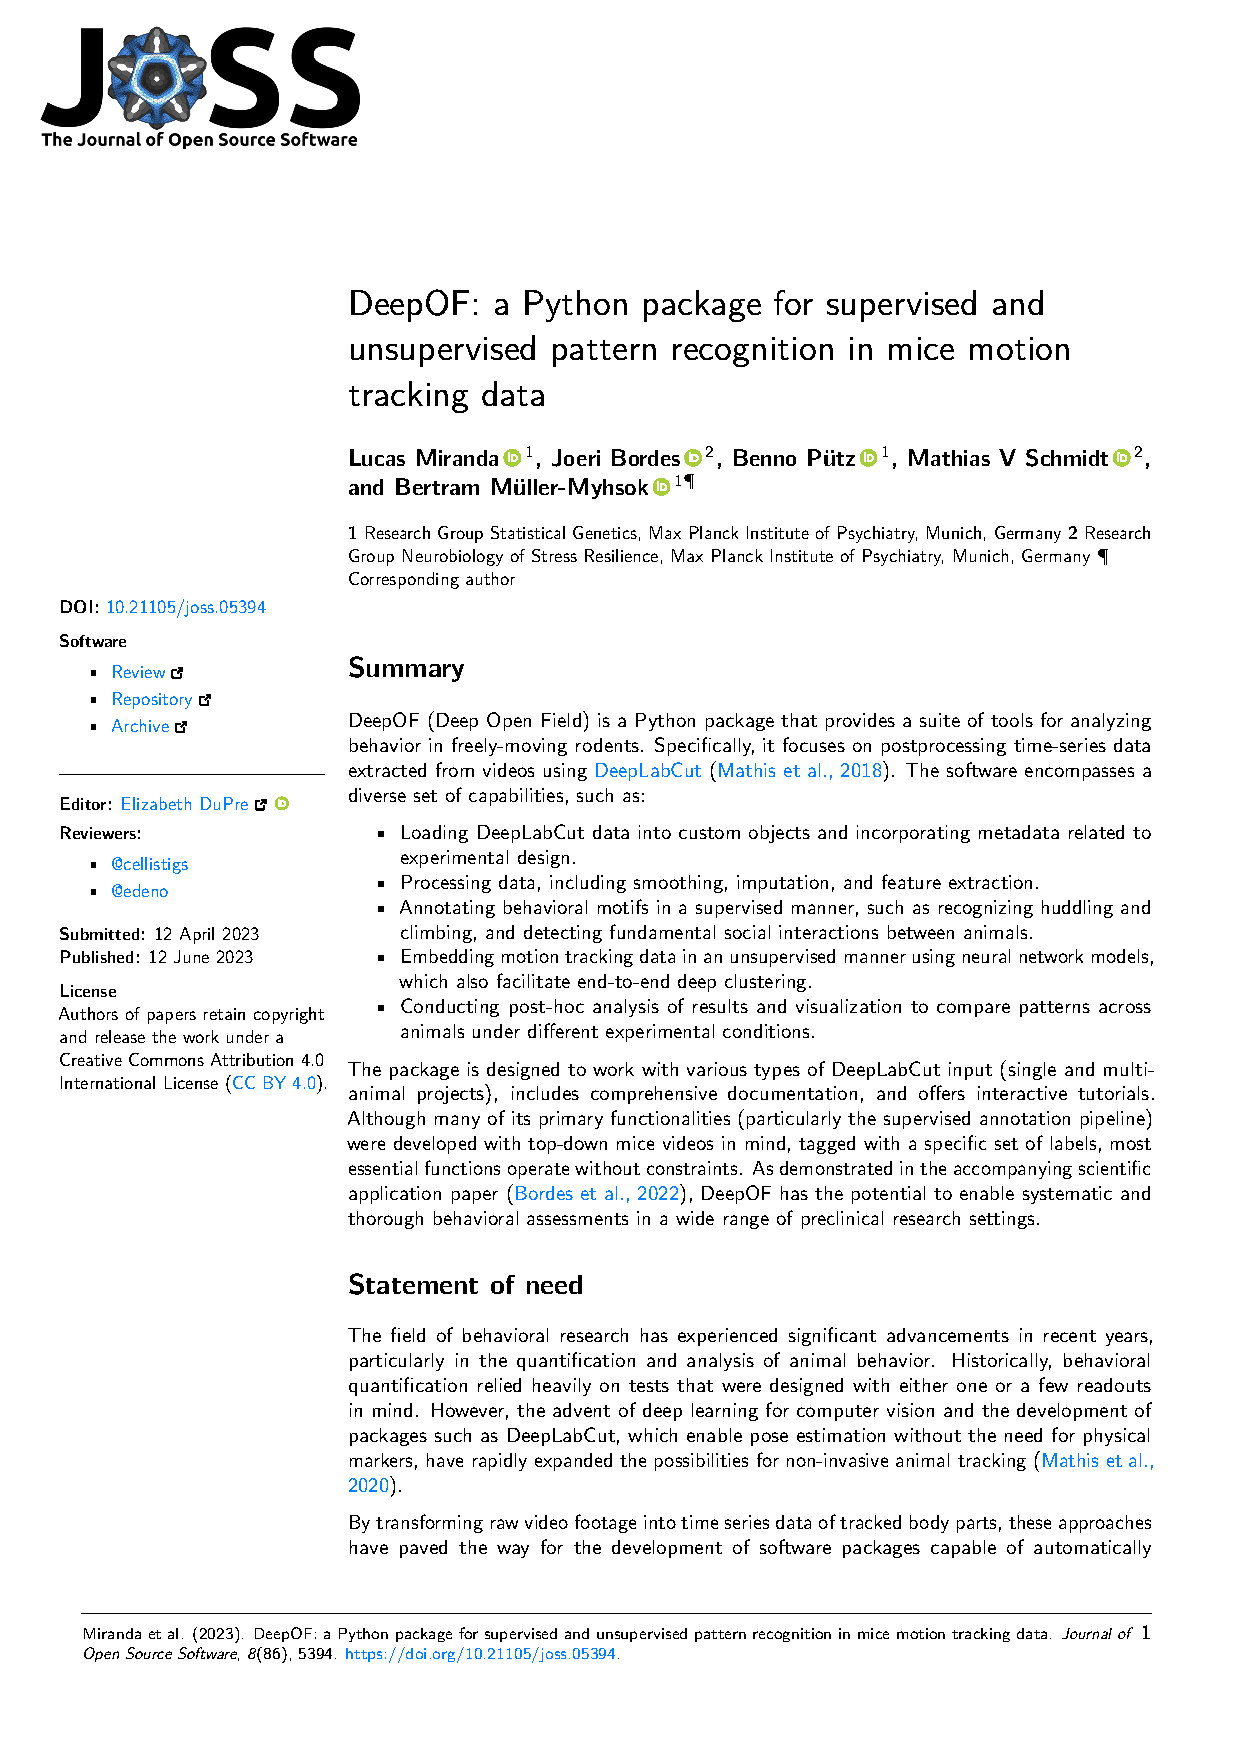
\includepdf[
            pages={-},
            addtolist={2, figure, \textbf{Schematic representation of the DeepOF workflow}, joss:fig1}
            ]{Papers/joss.pdf}